\documentclass[11pt]{article}
\usepackage{amsmath,amsthm,amssymb,fullpage,graphicx,hyperref,listings}
\usepackage{listings,color,setspace}
\author{Andy Reagan}
\title{Math 337 Homework 03 Rewrite}

     \def\NN{\mathbb{N} }
     \def\ZZ{\mathbb{Z} }
     \def\QQ{\mathbb{Q} }
     \def\RR{\mathbb{R} }
     \def\CC{\mathbb{C} }
     \def\f{\frac }
     \def\b{\begin }
     \def\e{\end }
     \def\Log{\text{Log} \,}
     \def\Re{\text{Re} \, }

\lstset{language=MATLAB,
basicstyle=\ttfamily\scriptsize\singlespacing,
keywordstyle=\color{blue},
stringstyle=\color{red},
commentstyle=\color{green},
morecomment=[l][\color{magenta}]{\#},
frame=L,
xleftmargin=\parindent,
%%numbers=left,                   %% where to put the line-numbers
%%numberstyle=\scriptsize,      %% the size of the fonts that are used for the line-numbers
%%stepnumber=1,                   %% the step between two line-numbers. If it is 1 each line will be numbered
numbersep=5pt,
breaklines=true,        %% sets automatic line breaking
breakatwhitespace=false,    %% sets if automatic breaks should only happen at whitespace
escapeinside={\%*}{*)} 
}


\newcommand{\pdiff}[2]{\frac{\partial #1}{\partial #2}}
\newcommand{\partialdiff}[2]{\frac{\partial #1}{\partial #2}}
\newcommand{\pdiffsq}[2]{\frac{\partial^2 #1}{{\partial #2}^2}}
\newcommand{\pdiffcu}[2]{\frac{\partial^3 #1}{{\partial #2}^3}}
     \newcommand{\pdiffhi}[3]{\frac{\partial^#3 #1}{{\partial #2}^#3}}
     \newcommand{\diff}[2]{\frac{{\rm d}#1}{{\rm d}#2}}
     \newcommand{\diffsq}[2]{\frac{{\rm d}^{2}#1}{{\rm d} {#2}^2}}
     \newcommand{\diffhi}[3]{\frac{{\rm d}^#3 #1}{{\rm d} {#2}^#3}}
     \newcommand{\tdiff}[2]{\mbox{d} #1/\mbox{d} #2}
     \newcommand{\tdiffsq}[2]{\mbox{d}^{2} #1/\mbox{d} {#2}^2}
     \newcommand{\tpdiff}[2]{\partial #1/\partial #2}
     \newcommand{\tpdiffsq}[2]{\partial^2 #1/\partial {#2}^2}
     \newcommand{\bvec}[1]{\vec{ {\bf #1 } }}

\begin{document}
\maketitle

\begin{enumerate}

\item Using Taylor expansions of $y'_{i-1}$ and $y'_{i-2}$ about $x = x_i$, verify that
\[ y_i ''' = \f{y_i'-2y_{i-1}'+y_{i-2}'}{h^2} + O(h) . \]

\bigskip
\textbf{Solution:} Using the Taylor expansions, we have 
\begin{align} y_{i-1} ' = y_i ' - h y_i '' + \f{h^2}{2} y_i ''' + O(h^3) \\
-2 y_{i-1} ' = -2 y_i ' + 2 h y_i '' - h^2 y_i ''' + O(h^3) \\
y_{i-2} ' = y_i ' - 2 h y_i '' + 2 h^2y_i ''' + O(h^3) \end{align}
Using these expansions, notice that the $y_i$ and $hy_i$ terms cancel as follows
\begin{align} -2y_{i-1}'+y_{i-2}' &= -y_i + h^2 y_i''' + O(h^3)\end{align}
such that
\begin{align} \f{y_i'-2y_{i-1}'+y_{i-2}'}{h^2} &= \f{h^2y_i'''+O(h^3)}{h^2} = y_i''' + O(h), \end{align}
as desired.
\item[4] Use the Predictor-Corrector method given by Eqs 3.33, 3.39, and 3.40 to solve
\begin{equation} y' = \sin y, ~~~~ y(0) = 1, ~~~~ x \in [0, \pi ] . \end{equation}
Select the step size so that the local truncation error, given by 3.39, be at most $\epsilon _{\text{loc}} = 10^{-4}$.
Provide an  explanation for your choice of the step size.

\bigskip
\textbf{Solution:} Using formula 1.28, the third derivative of $y$ is
\begin{align} y'''(x) &= f_{xx} + f_x f_y + 2f f_{xy} + f (f_y ) ^2 + f^2 f_{yy} \end{align}
I compute the respective derivatives as
%% \begin{align} f_{x} &= \pdiff{f}{x} + \pdiff{f}{y} \diff{y}{x} \\
%% &= \cos(y(x)) \sin(y(x)) + \cos(y(x)) \sin(y(x)) = 2\cos(y(x)) \sin(y(x)) \\
%% f_{xx} &= \pdiff{f_x}{x} + \pdiff{f_x}{y} \diff{y}{x}\\
%% &= 2 \cos ^2 (y(x)) \sin (y(x)) - 2 \sin ^3 (y(x)) + ( 2\cos ^2 (y(x)) - 2\sin ^2 (y(x))) \sin (y(x))\\
%% &= 4 \cos ^2 (y(x)) \sin (y(x)) - 4 \sin ^3 (y(x))\\
%% f_y &= \pdiff{f}{y} + \pdiff{f}{x} \diff{x}{y}\\
%% &= \cos (y(x)) + \cos(y(x)) \sin(y(x)) \cdot 0 = \cos (y(x))\\
%% f_{yy} &= \pdiff{f_y}{y} + \pdiff{f_y}{x} \diff{x}{y}\\ 
%% &= -\sin(y(x)) \\
%% f_{xy} &= \pdiff{f_x}{y} + \pdiff{f_x}{x} \diff{x}{y}\\
%% &= 2\cos ^2 (y(x)) - 2 \sin ^2 (y(x)) \end{align}
\begin{align} f_{x} &= \cos (y(x)) \sin (y(x)) \\
f_{xx} &= \cos (y(x)) \cos (y(x)) \sin (y(x)) + \sin (y(x)) (-\sin(y(x)) \sin(y(x)))\\
&= \cos ^2(y(x)) \sin (y(x)) - \sin ^3 (y(x)) \\
f_y &= \cos (y(x))\\
f_{yy} &= -\sin(y(x)) \\
f_{xy} &= \cos ^2 (y(x)) - \sin ^2 (y(x)) \end{align}

Therefore we have
%% \begin{align} y'''(x) &= 4 \cos ^2 (y(x)) \sin (y(x)) - 4 \sin ^3 (y(x)) + 2\cos(y(x)) \sin(y(x)) \cos (y(x)) \\
%% &+2 \sin (y(x)) \left [2\cos ^2 (y(x)) - 2 \sin ^2 (y(x)) \right ] + \sin (y(x)) \cos^2 (y(x)) - \sin^3 (y(x)) \end{align}
\begin{align} y'''(x) &= \cos ^2(y(x)) \sin (y(x)) - \sin ^3 (y(x)) + \cos ^2(y(x)) \sin (y(x)) \\
&+ 2\sin (y(x)) (\cos ^2 (y(x)) - \sin ^2 (y(x))) + \sin (y(x)) \cos ^2 (y(x)) - \sin ^2 (y(x)) \sin (y(x))\\
&=5 \cos ^2(y(x)) \sin (y(x)) - 3\sin ^3 (y(x)) \end{align}

I'm not confident in this equation, so I set the max of $y'''$ to 1 per our discussion.
With the error given by Equation 3.39, we compute $h$ for $\epsilon _\text{loc} = 10^{-4}$ and choose the max of $y'''(x)$ on $[0,\pi]$.
For the max of $y'''$ set to 1, we find $h = 0.1062$.


In Figure 1, we plot the numerical solution.
We test whether our timestep controlled the error in Figure 2.
We see that the error estimate which we made was sufficient to contain the error within $\epsilon _\text{loc} = 10 ^{-4}$.

The step size computation, shown in the code, is equivalent to solving 3.37 with our estimate of $y'''$ given above:

\[ |\epsilon_{i+1} | \approx 1/12 \cdot h^3 | y''' _{i+1}| ~~~~~~~~~\Rightarrow~~~~~~~~ h \approx \sqrt[3]{12 |\epsilon_{\text{loc}}| / | y''' _{i+1}|} .\]

\lstinputlisting[language=Matlab]{andy_hw03_prb4_2.m}

\begin{figure}
  \centering
    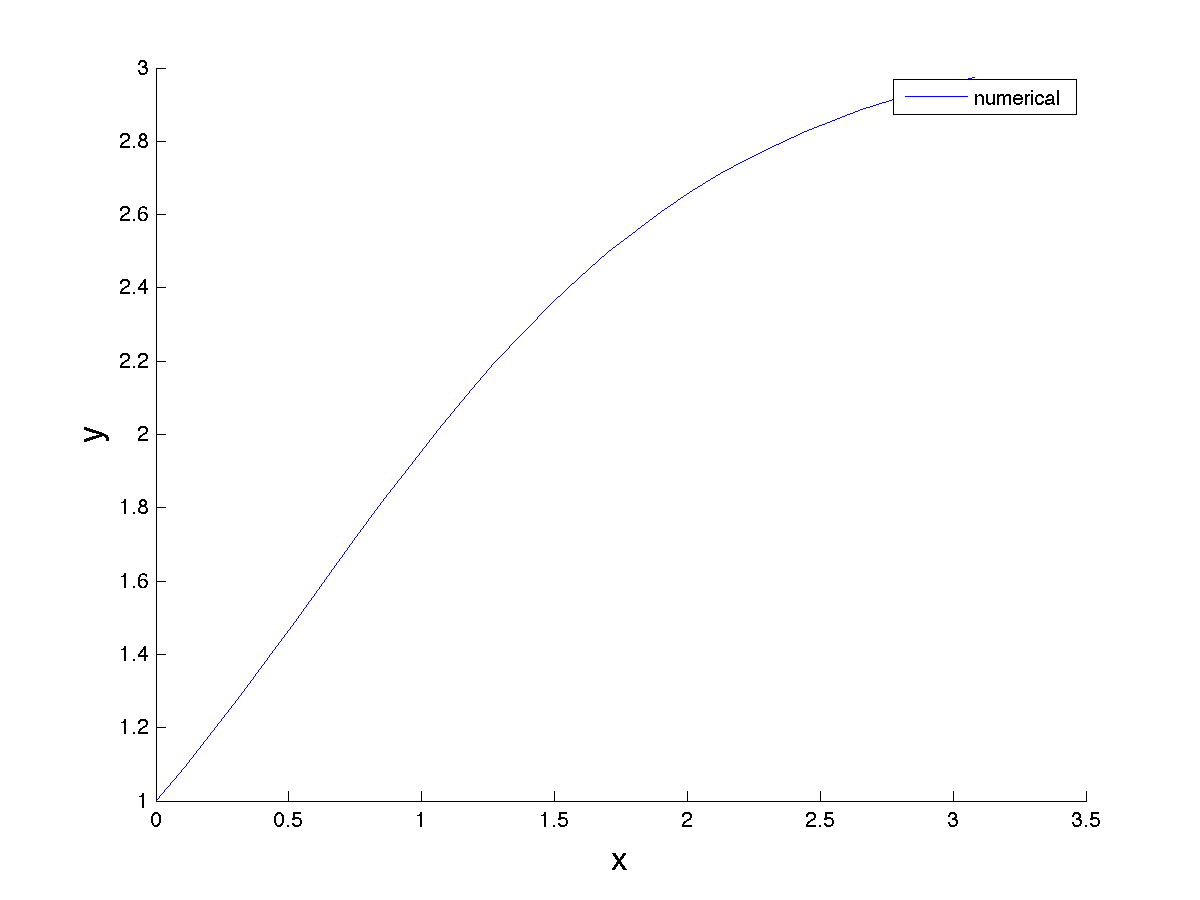
\includegraphics[width=0.6\textwidth]{andy_hw03_prb4_numerical.png}
  \caption{The numerical solution.}
\end{figure}

\begin{figure}
  \centering
    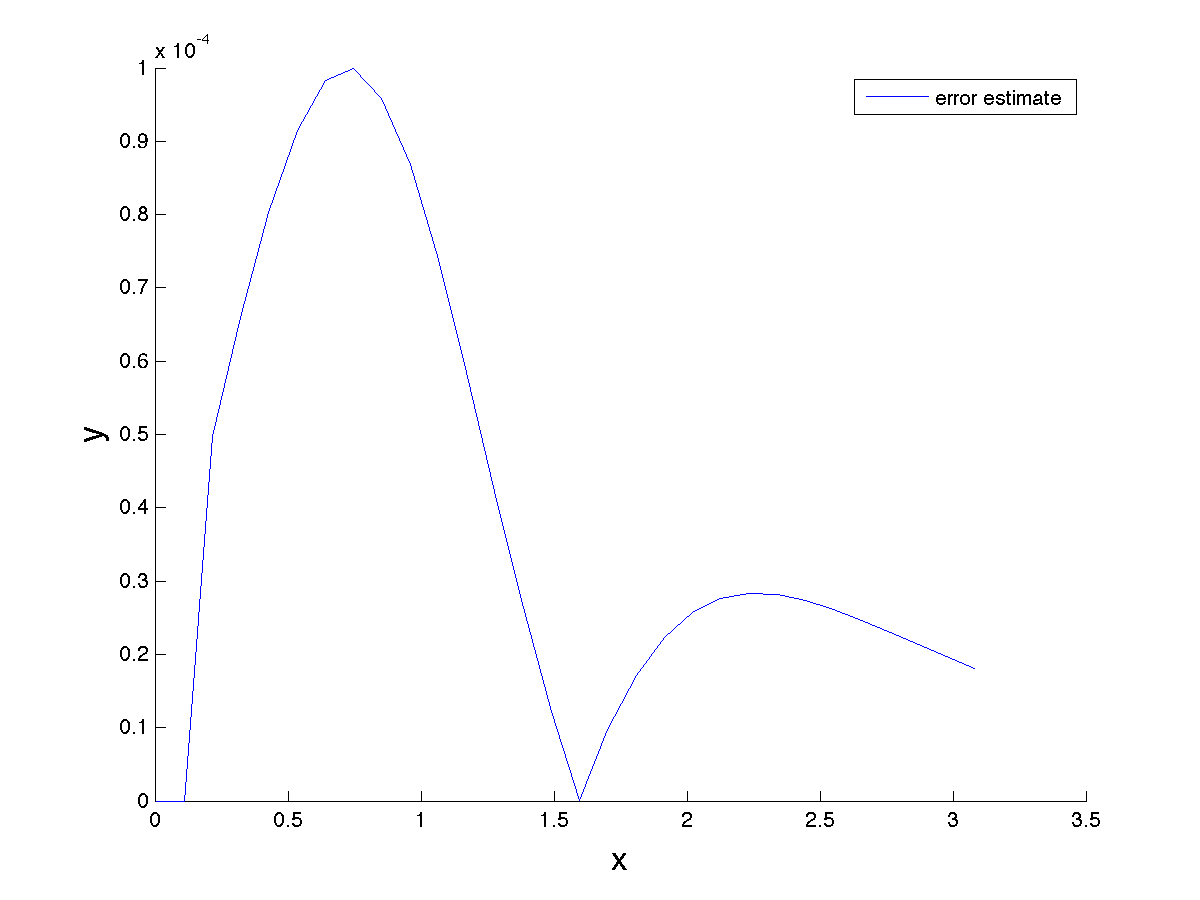
\includegraphics[width=0.6\textwidth]{andy_hw03_prb4_just_error.png}
  \caption{The estimated error at each time step.}
\end{figure}

\end{enumerate}



\end{document}
